\chapter{Evaluation}
\label{chap:evaluation}

\subsection{Preface}

To evaluate the different controllers, multiple tests showing off their individual strengths and weaknesses were done. All of the controllers were tested multiple times to get a good sample size, the data was treated and cleaned, and then a set of data deemed to be the most representative was chosen for each controller and for each test. All the data can be found in REF[] but graphs of the representative data can be seen here. \\

For each test, 3 graphs were made. The cart position shows how the cart reacts and moves during the various stages of tests. Because 0 is in the center of the track, the graphs will always be centered around that, as all units are in the treated units and not in raw encoder units. The pendulum angle shows what the angle of the entire pendulum is during the tests. This is shown in degrees measured by the encoder sitting at the base of the pendulum in the carts center. The motor force test is readout of the force applied by the motor. It is measured in newtons, as the motor drive has a mode specifically for torque, as mentioned in REF[]. 

All the tests are colour-coded, and the simulation tests from SIMULINK are the same colour as the physical test, but a dotted.

\subsection{Impulse test}

The impulse test was done by applying a single impulse of 6 newtons, for 50 milliseconds, to the output of the controller. This means that at an output of 1 newton, would mean that the cart would be affected by 6 newtons for 50 milliseconds. It is primarily used to show how the various controllers recover from one off pushes.

\begin{figure}[H]
    \centering
	
\includegraphics[width=1.0\textwidth]{Figures/Impulse_cart_pos.png}
	\caption{Cart position during the impulse test.}
	\label{fig:impulse_cart_pos}   
\end{figure}

\begin{figure}[H]
    \centering
	
\includegraphics[width=1.0\textwidth]{Figures/Impulse_pend_angle.png}
	\caption{Pendulum angle during the impulse test.}
	\label{fig:impulse_pend_angle}   
\end{figure}

\begin{figure}[H]
    \centering
	
\includegraphics[width=1.0\textwidth]{Figures/Impulse_motor_u.png}
	\caption{Motor force during the impulse test.}
	\label{fig:impulse_motor_u}   
\end{figure}


\subsection{Step response test}

The step test was done similarly to the impulse, but instead it was applied for 10 seconds rather than 50 milliseconds, and with 8 newtons of force. This allows certain controllers to show off their resilience under continued pressure.

\begin{figure}[H]
    \centering
	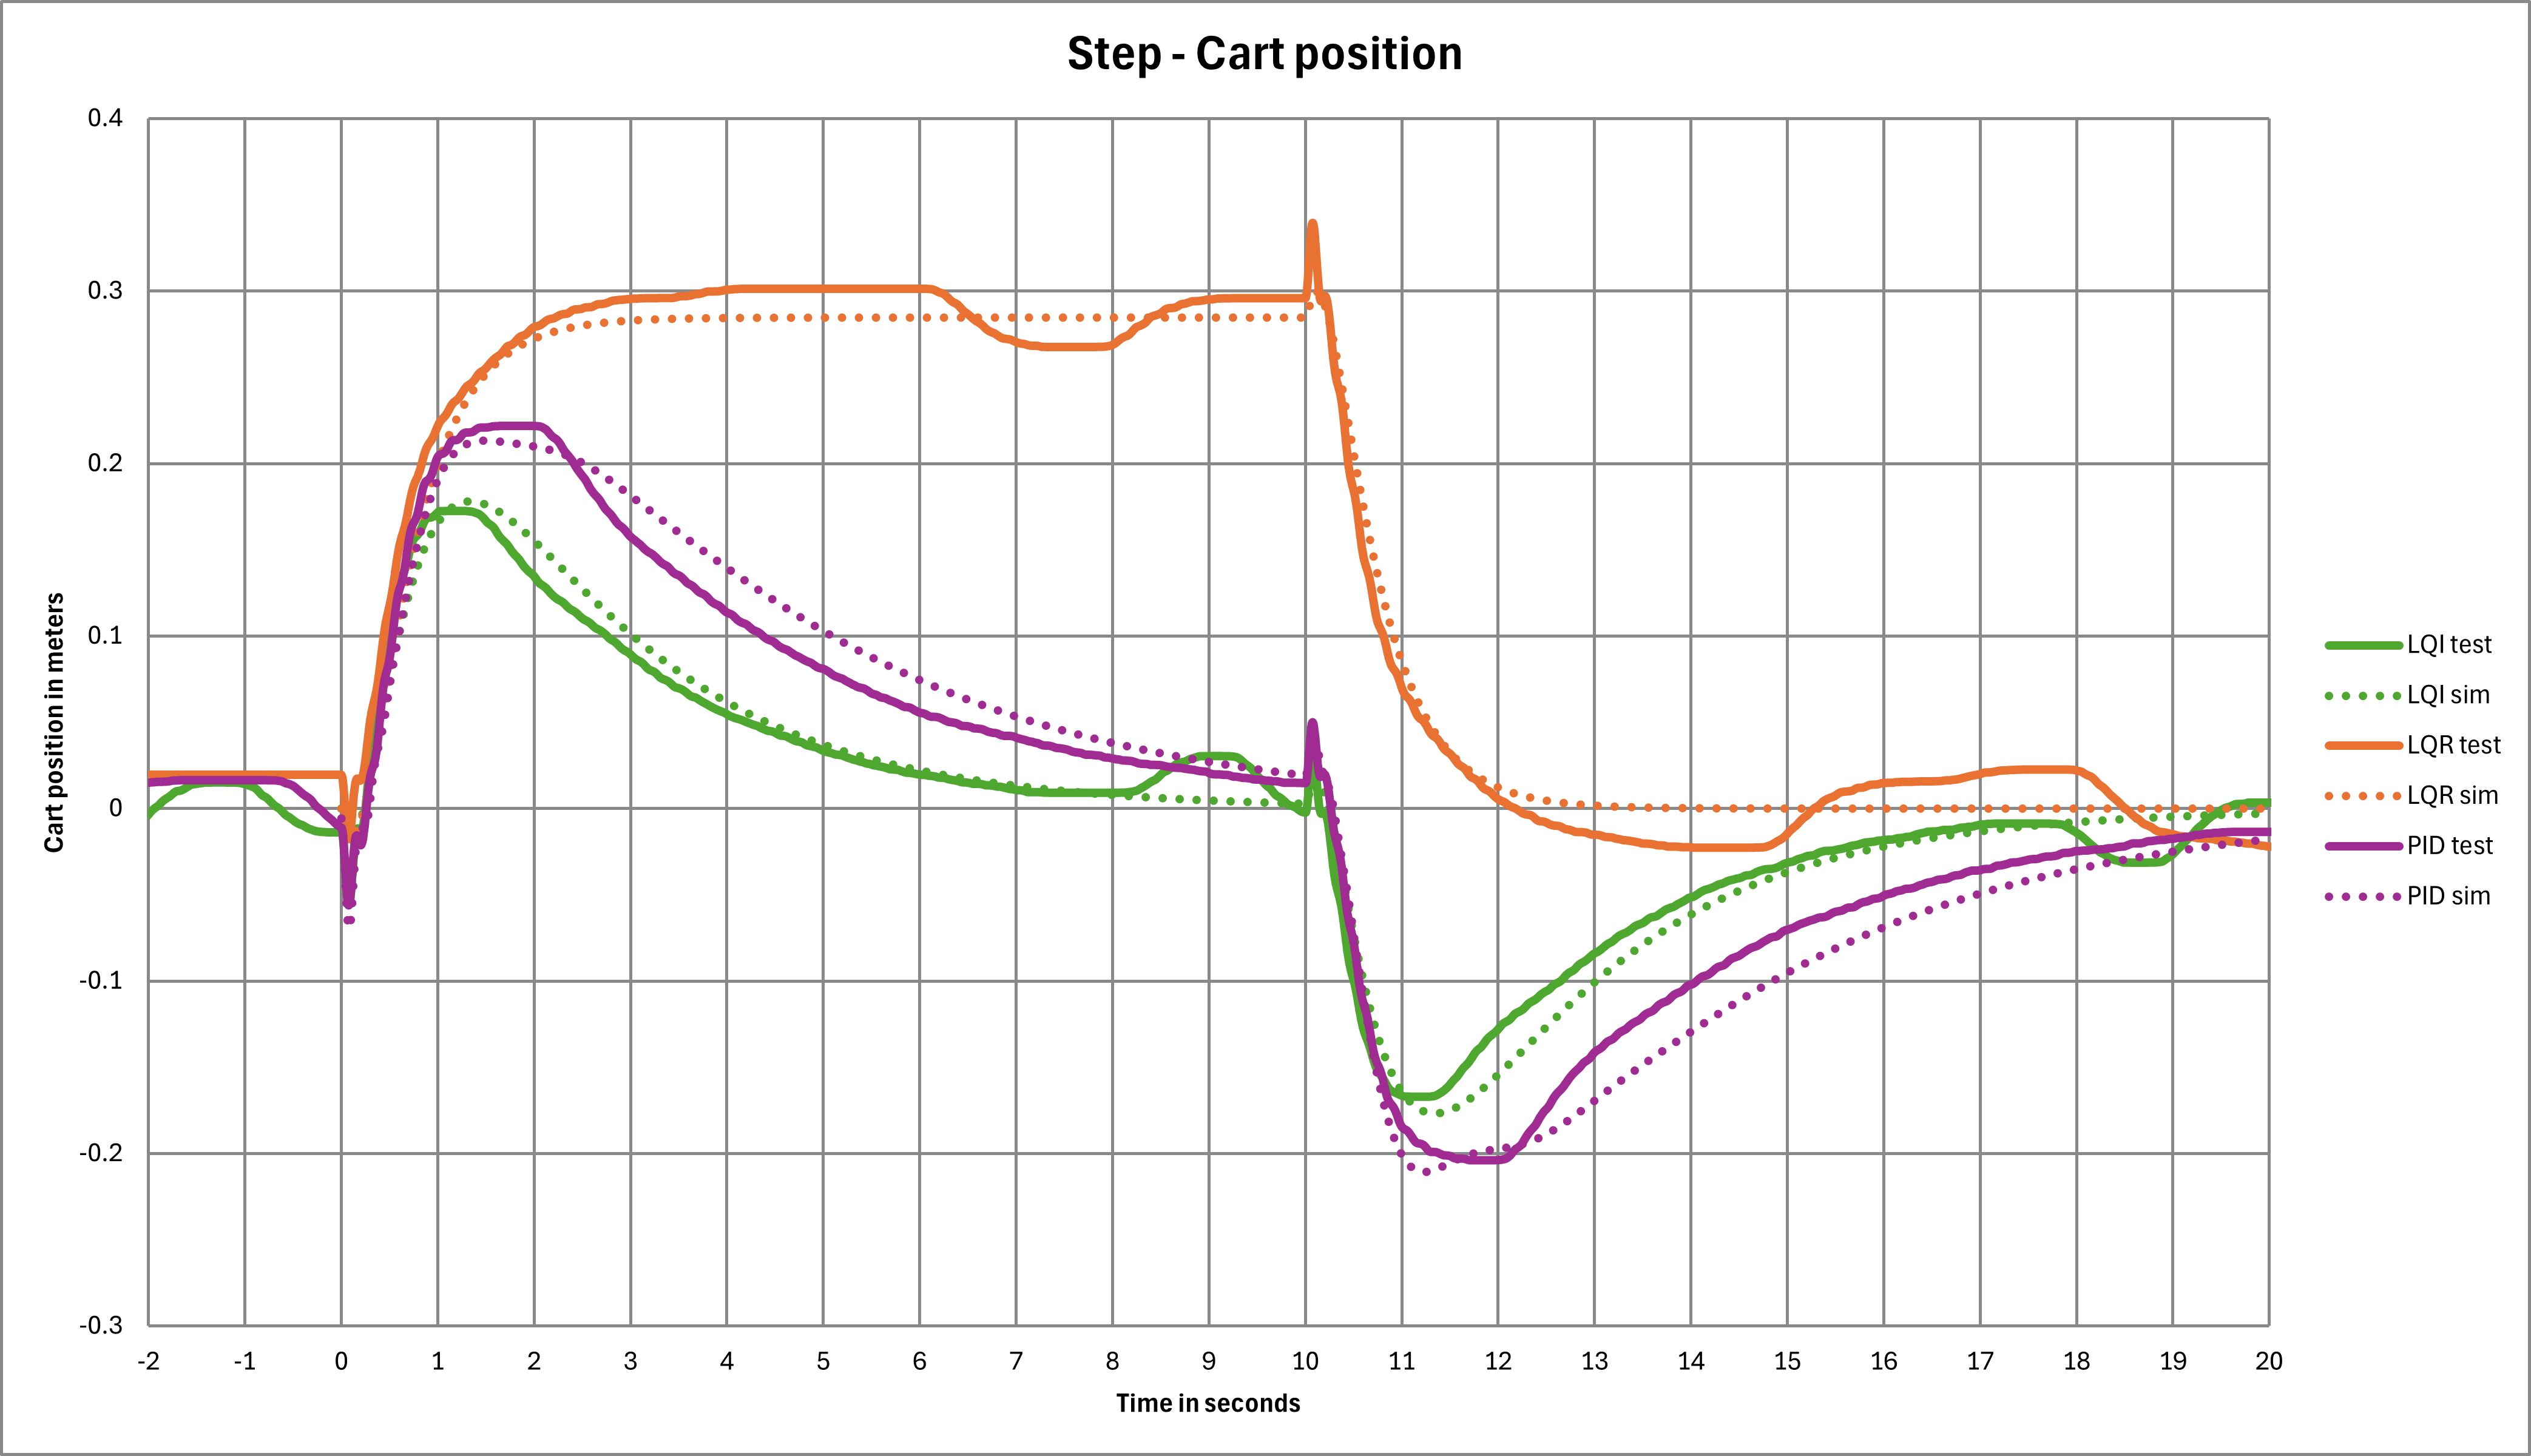
\includegraphics[width=1.0\textwidth]{Figures/Step_cart_pos.png}
	\caption{Cart position during the step response test.}
	\label{fig:Step_cart_pos}   
\end{figure}

\begin{figure}[H]
    \centering
	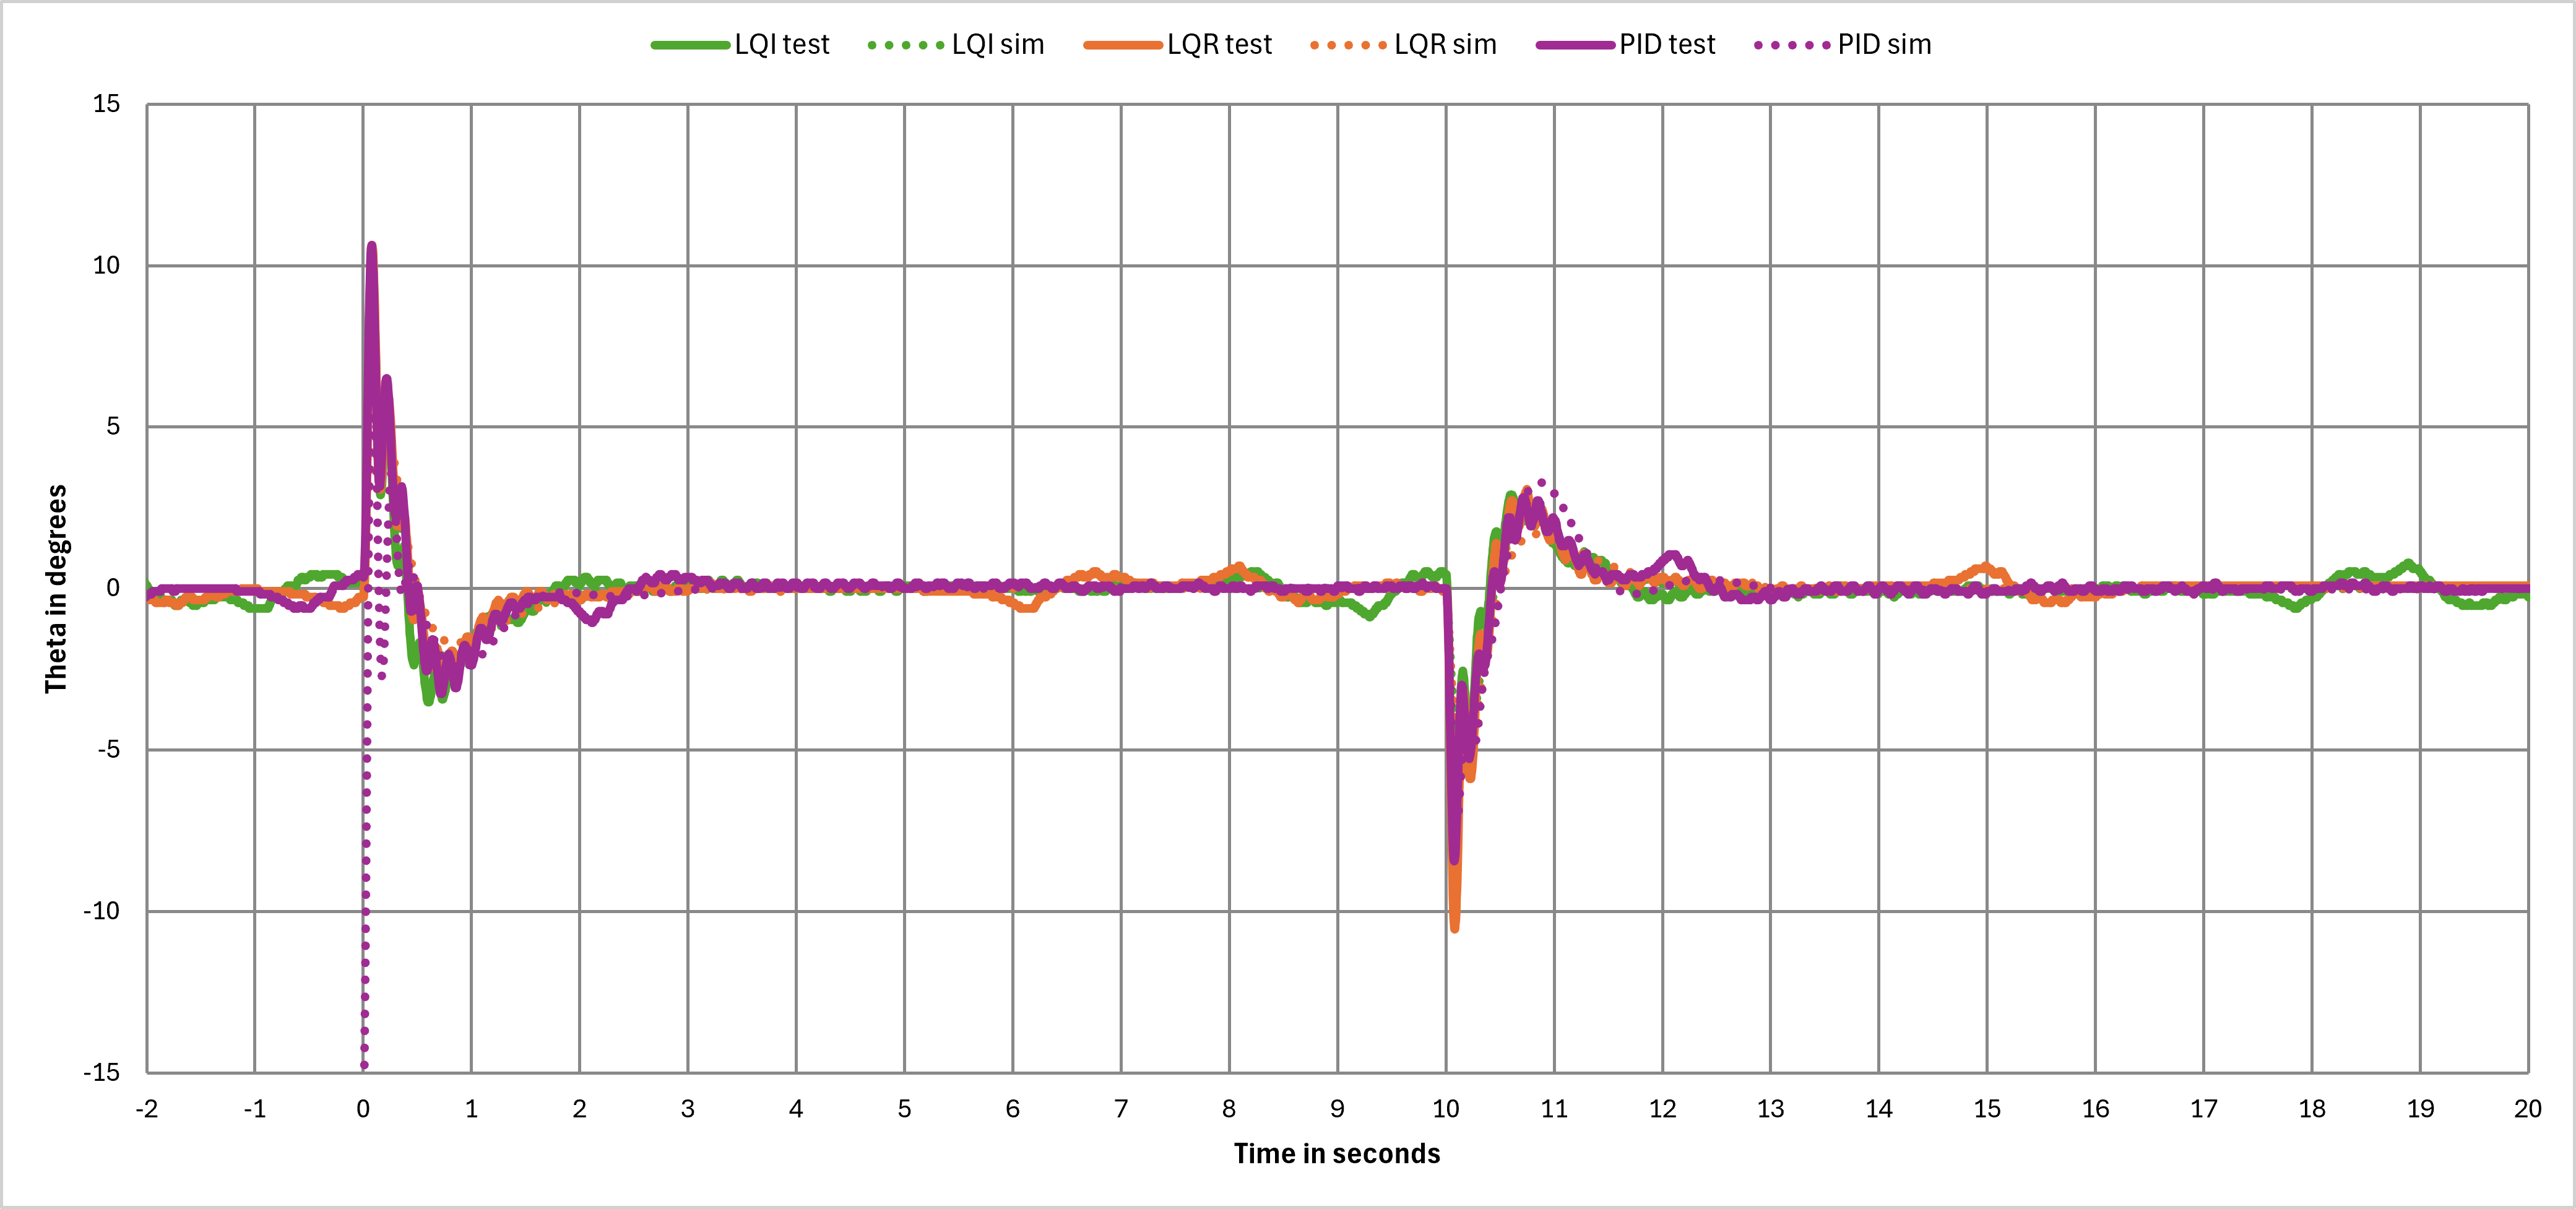
\includegraphics[width=1.0\textwidth]{Figures/Step_pend_angle.png}
	\caption{Pendulum angle during the step response test.}
	\label{fig:Step_pend_angle}   
\end{figure}

\begin{figure}[H]
    \centering
	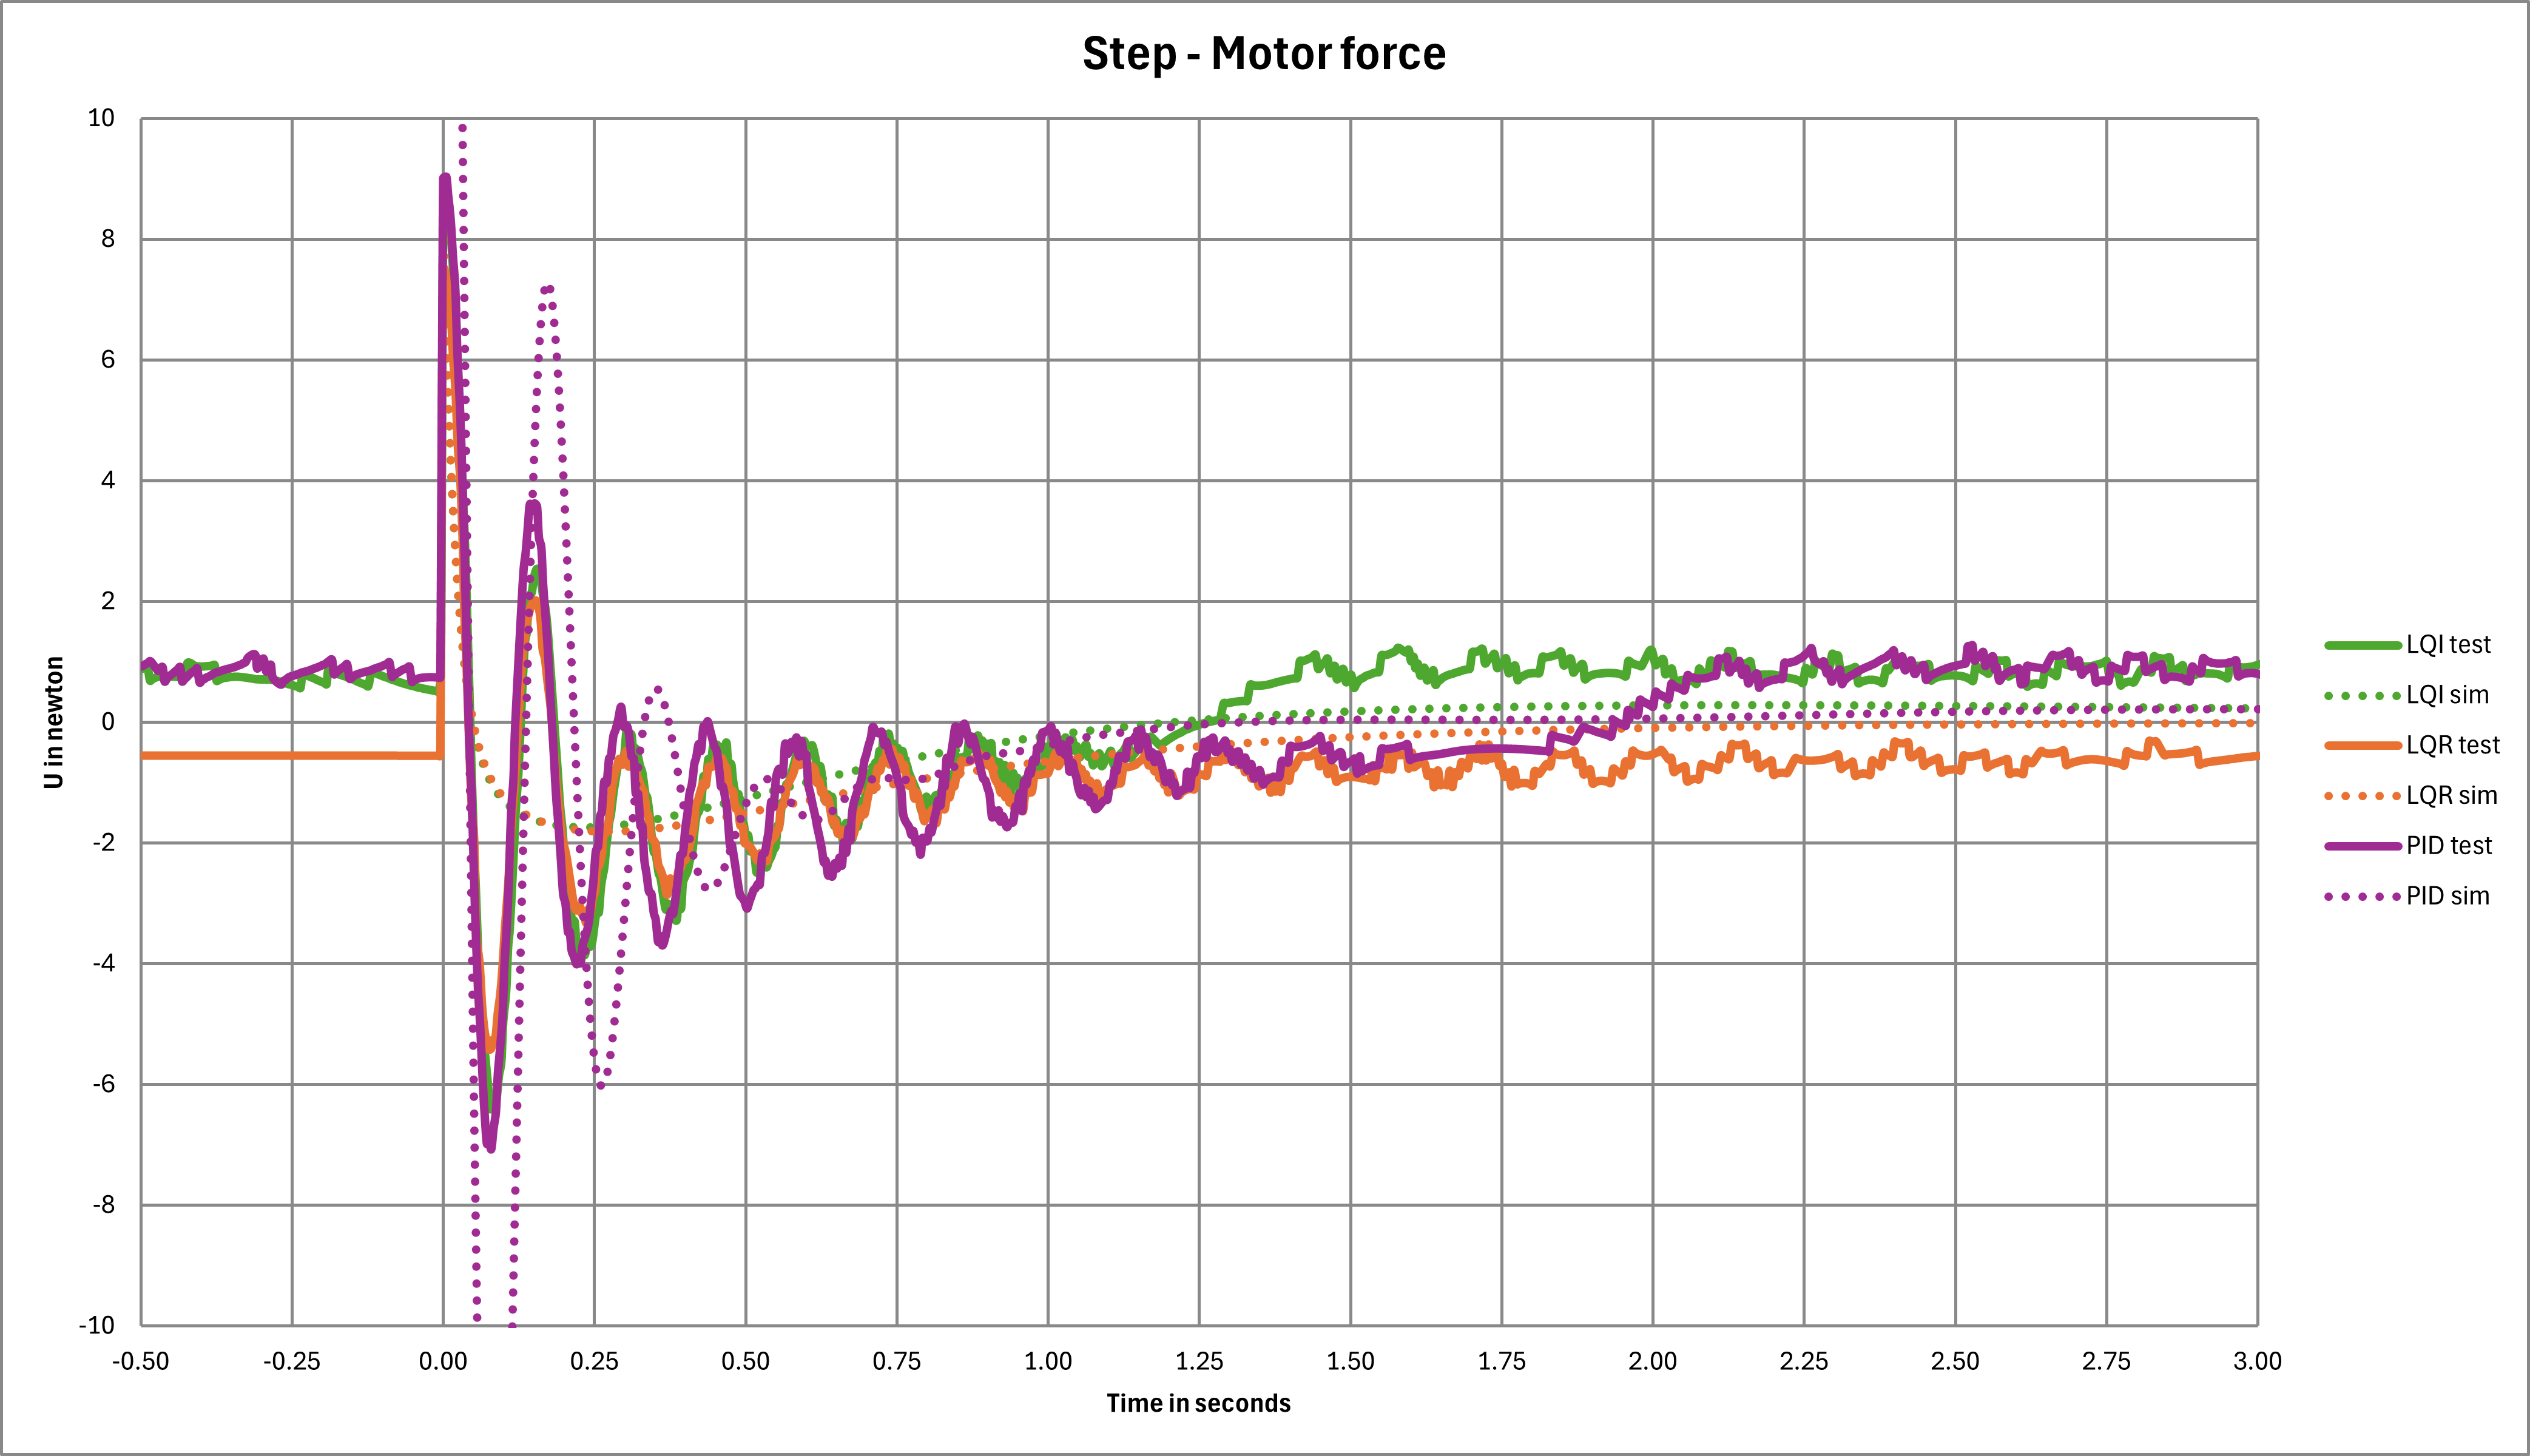
\includegraphics[width=1.0\textwidth]{Figures/Step_motor_u.png}
	\caption{Motor force during the step response test.}
	\label{fig:Step_motor_u}   
\end{figure}


\subsection{Swing up test}

Finally the swing up test, which was done by initiating the swing up, and switching to the controller when possible. This shows how quickly and well the controller can activate, stabilizing an unstable pendulum, and catching it when it reaches the top with a velocity that would allow the given controller to catch it. One thing to note is that the graphs only show the time after the controller kicked in, and not during the swingup itself.

\begin{figure}[H]
    \centering
	
\includegraphics[width=1.0\textwidth]{Figures/Swing_cart_pos.png}
	\caption{Cart position during the swing up test.}
	\label{fig:Swing_cart_pos}   
\end{figure}

\begin{figure}[H]
    \centering
	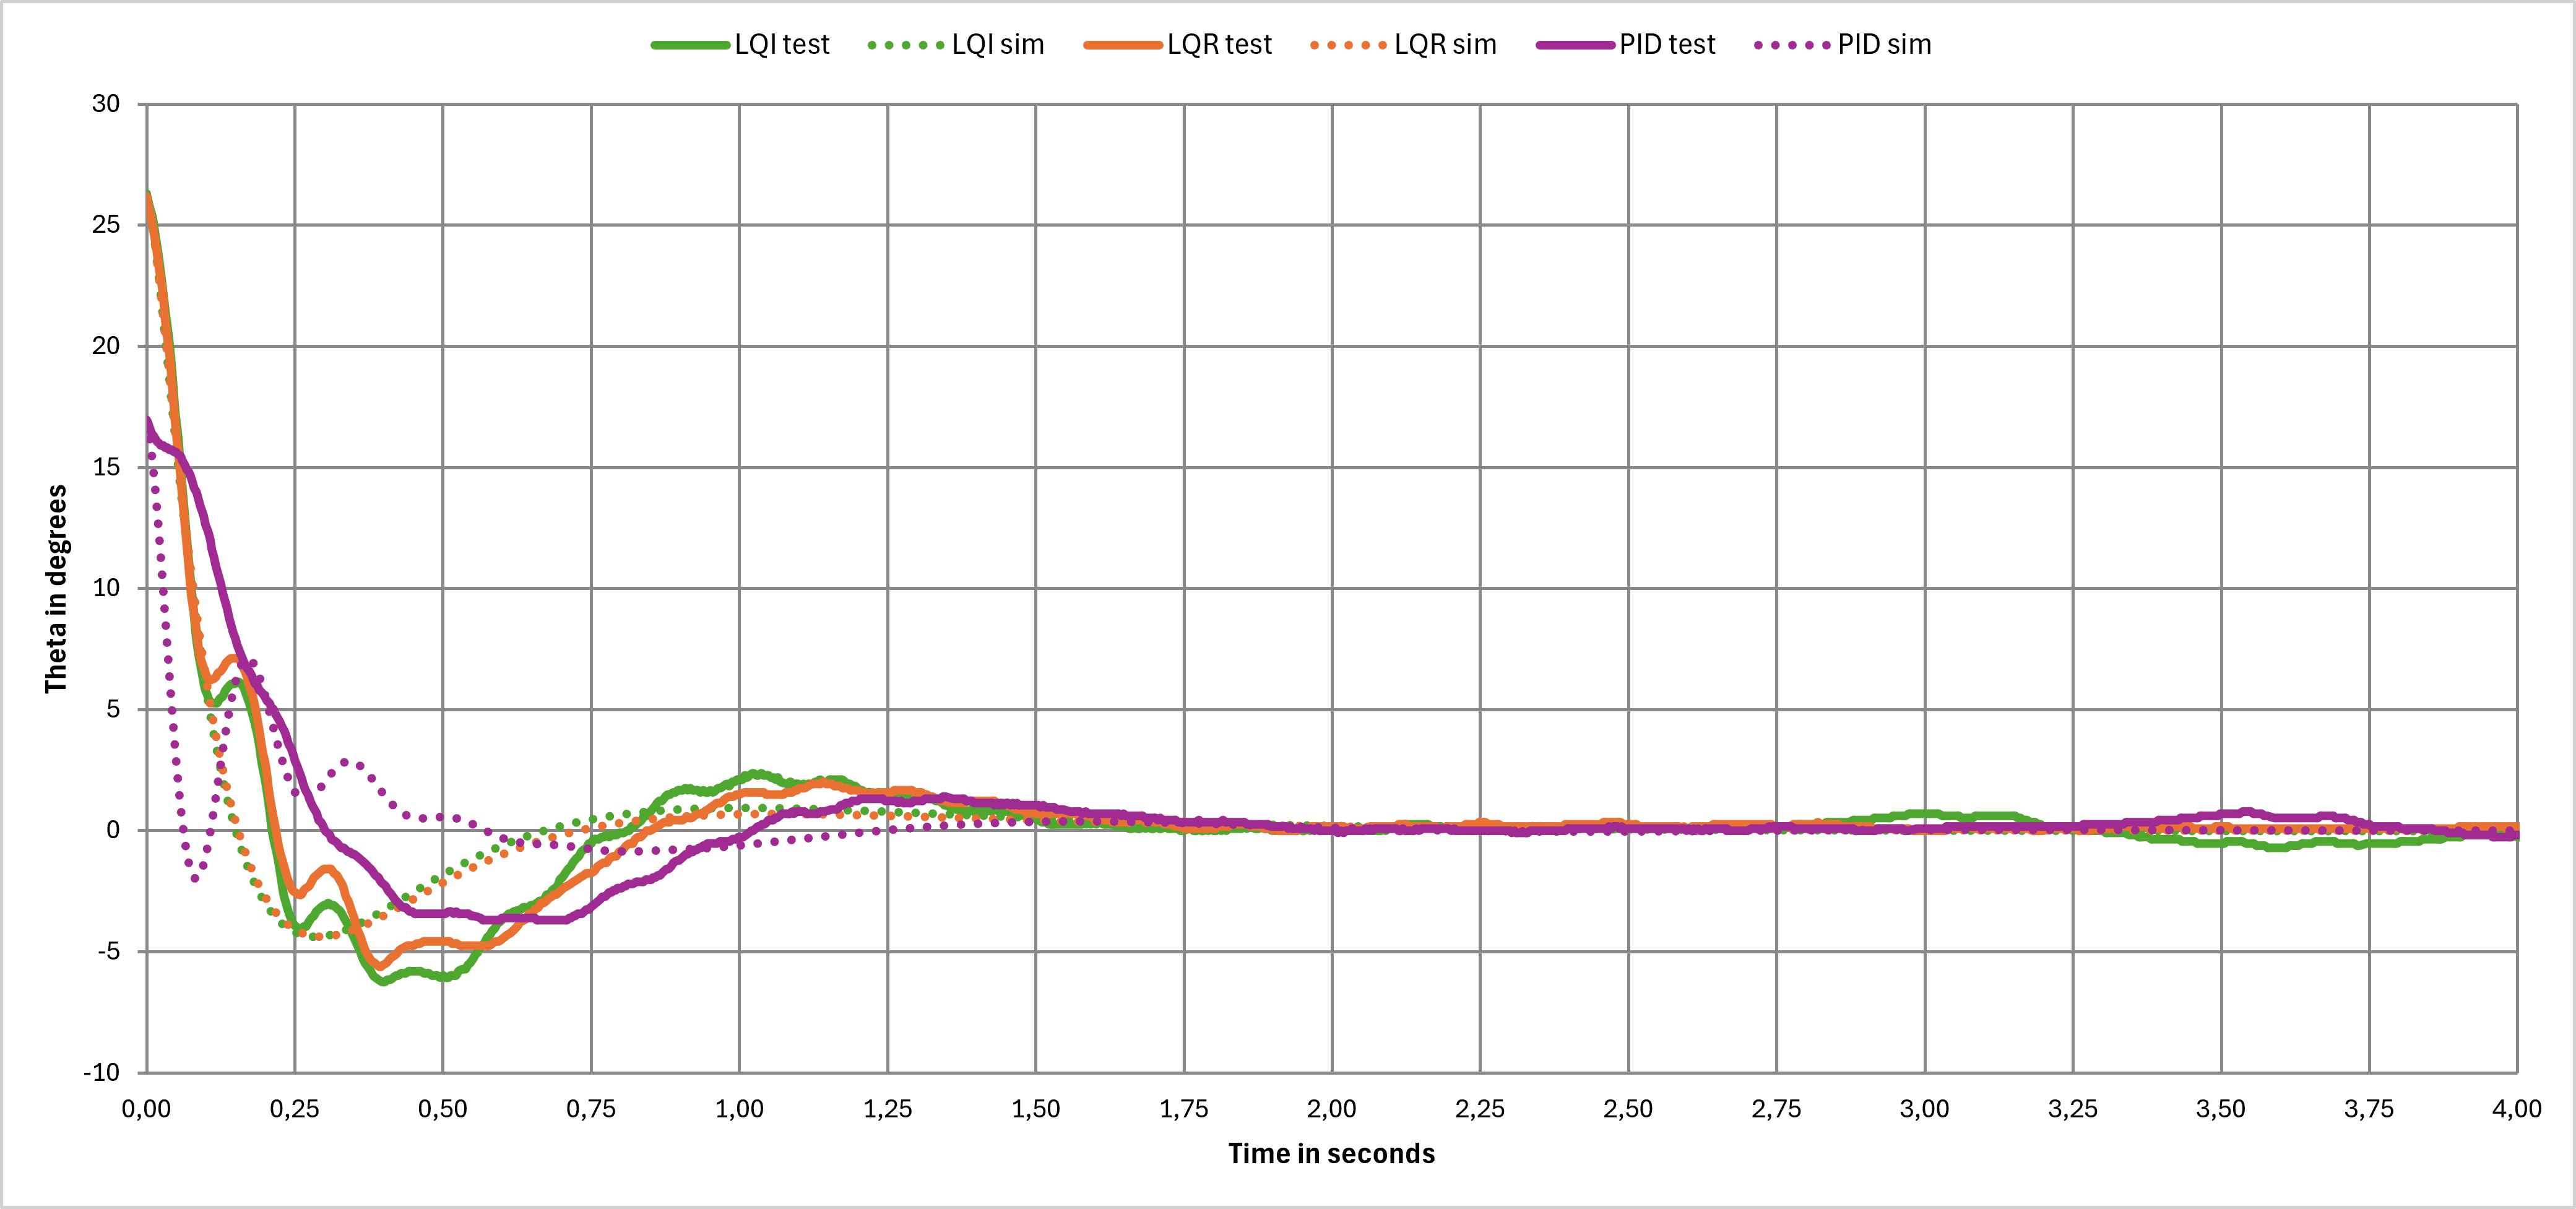
\includegraphics[width=1.0\textwidth]{Figures/Swing_pend_angle.png}
	\caption{Pendulum angle during the swing up test.}
	\label{fig:Swing_pend_angle}   
\end{figure}

\begin{figure}[H]
    \centering
	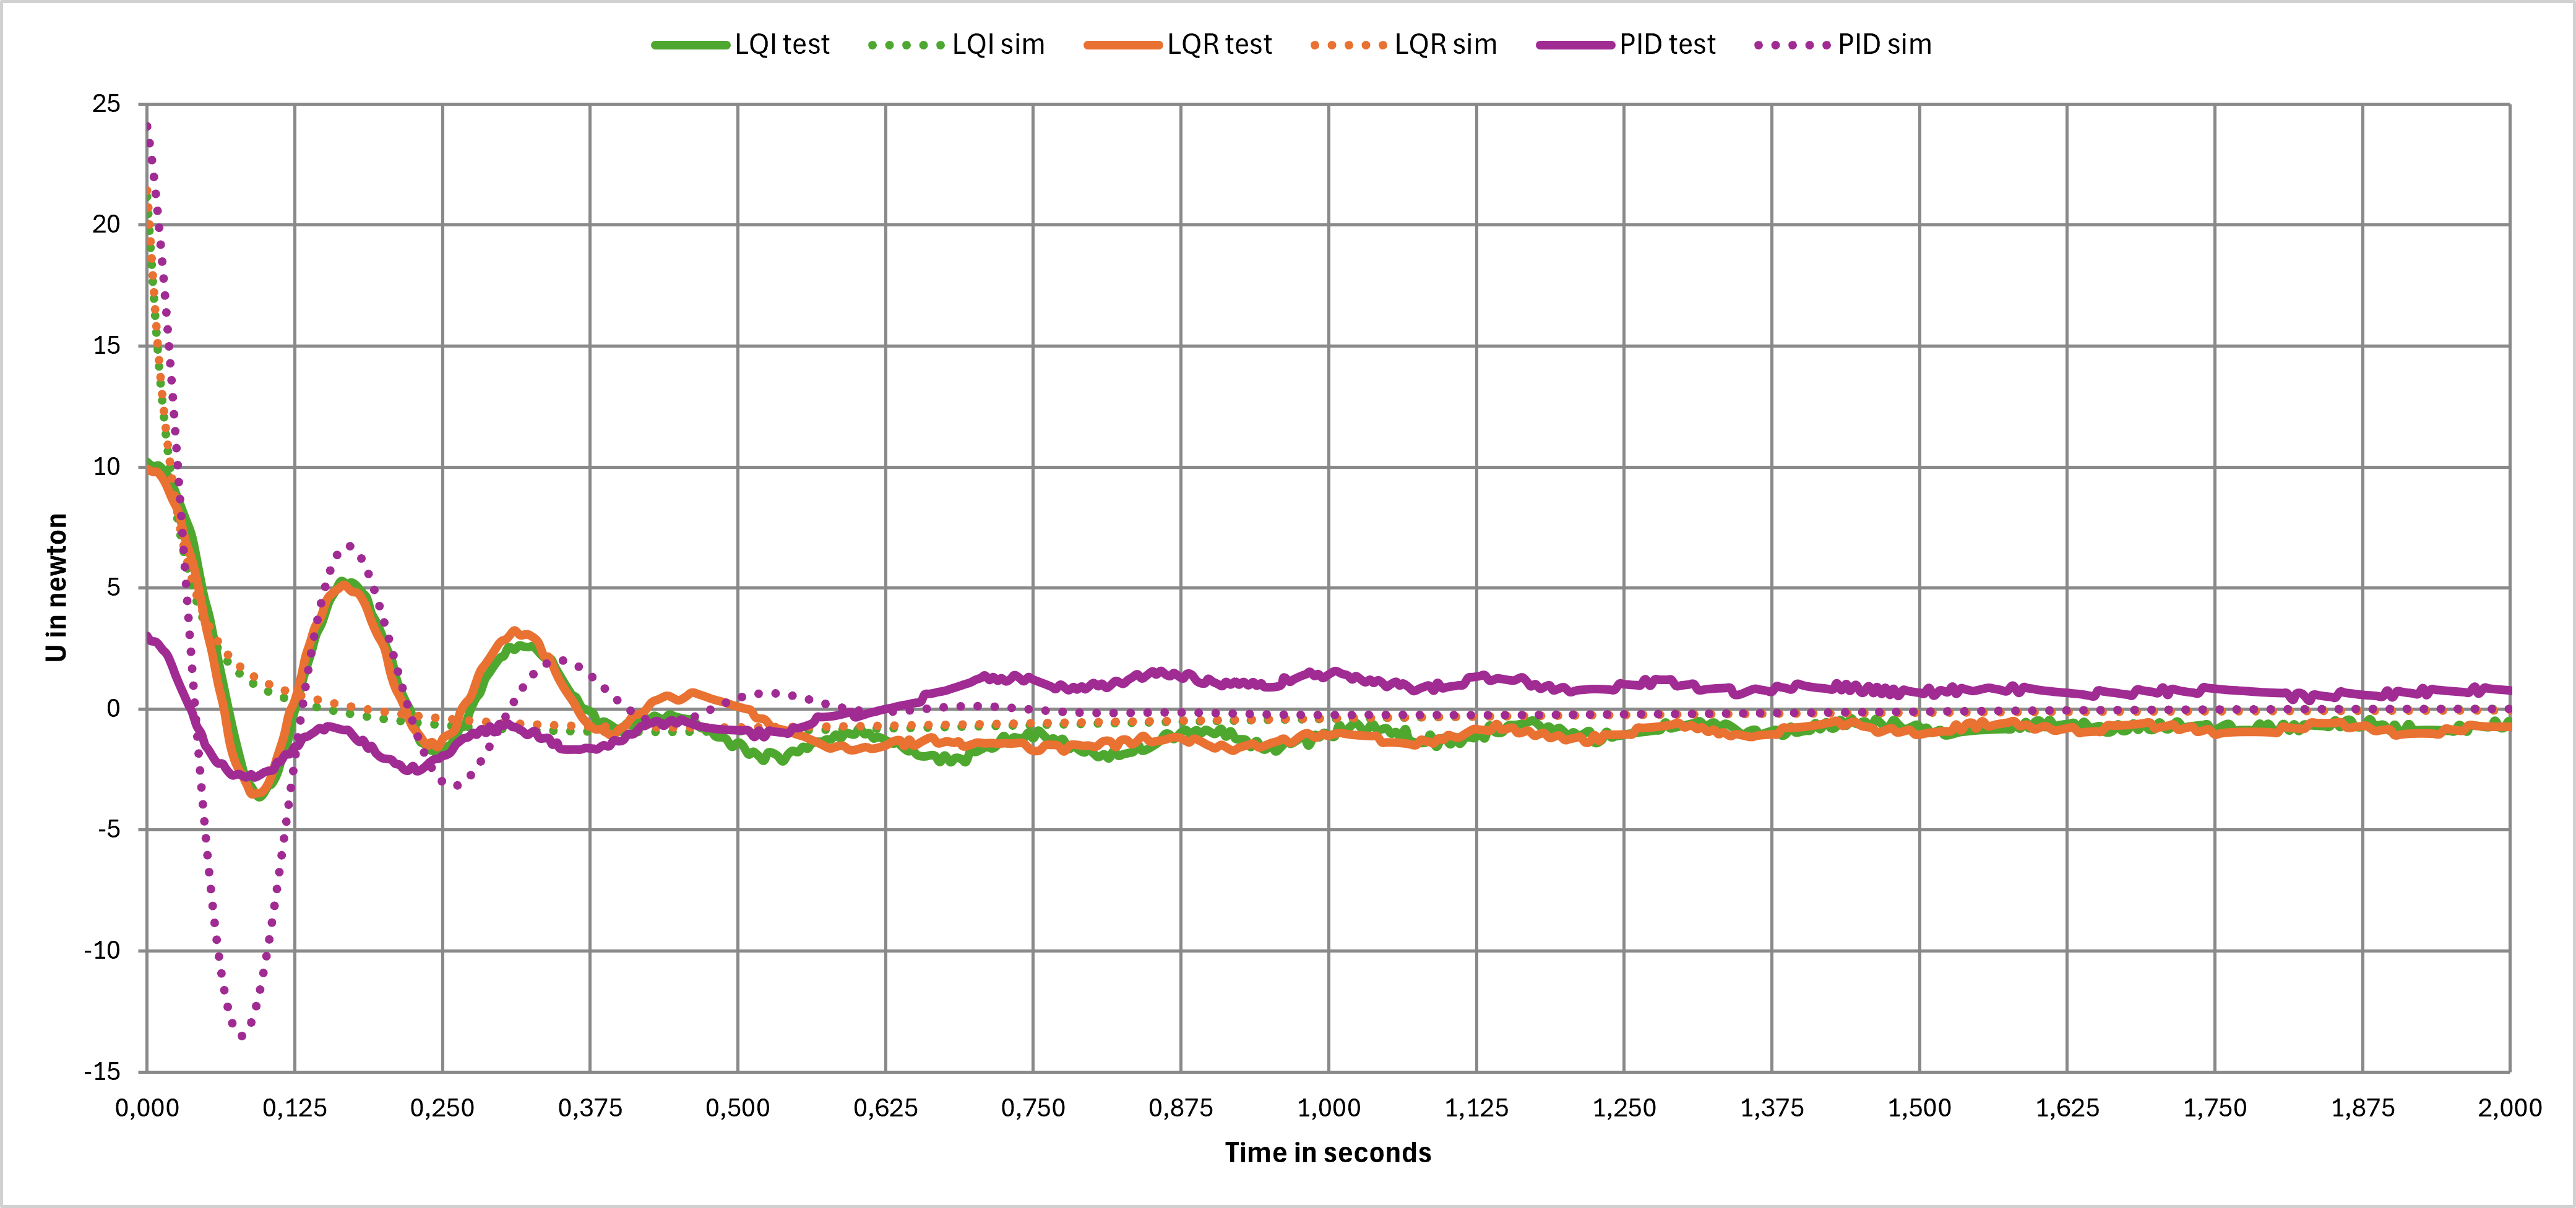
\includegraphics[width=1.0\textwidth]{Figures/Swing_motor_u.png}
	\caption{Motor force during the swing up test.}
	\label{fig:Swing_motor_u}   
\end{figure}